\section{Evaluation}
This section first presents the experimental setups and then assesses \system from the following aspects:
\begin{itemize}
    \item Evaluate whether \system improves query throughput while preserving recall when integrated with existing ANNS systems, and quantify its memory footprint (Section~6.2: Performance Study)
    \item Assess the impact of storage, validation, and index parameters on performance (Section~6.3: Parameter Study)
    \item Analyze \system’s behavior under larger update and query batches, increased dataset scales, and varying thread counts (Section~6.4: Scale-up Study)
\end{itemize}

\begin{table}[t]
    \centering
    \caption{Datasets used in evaluation}
    \label{tab:eval-datasets}
    \begin{tabular}{lcccc}
        \toprule
        Dataset & Type & Dimension & DataSize & QuerySize \\
        \midrule
        SIFT & Image &128 & 1,000,000 & 10,000 \\
        Msong & Audio & 420 & 992,272 & 200 \\
        Glove & Text & 100 &  1,192,514 & 200 \\
        SIFT-10M & Image &128 & 10,000,000 & 10,000 \\
        \bottomrule
    \end{tabular}
\end{table}

\subsection{Experimental Setup}
\noindent \textbf{Test-bed.} Experiments are conducted on a Linux Server (Ubuntu 22.04) with two Intel Xeon Platinum 8368Q CPUs (each with 38 cores at 2.60GHz) and 512GB memory.

\noindent \textbf{Baselines.} We evaluate \system on CANDOR-Bench~\cite{Wang202627} by deploying it on three representative ANNS systems and comparing their performance with and without \system under the same dynamic benchmark protocol. We select these baselines to cover complementary characteristics: (1) HNSW~\cite{Malkov2020824}, one of the most widely-used ANNS systems;
(2) SymphonyQG~\cite{Gou2025}, a recent static ANNS system that combines graph index with RabitQ quantization, representing static optimization approaches; and 
(3) FreshDiskANN~\cite{Singh2021}, a dynamic ANNS system for online updates, representing systems that natively handle dynamic workloads.
We denote the corresponding \system-enabled variants as HNSW-\system, SymphonyQG-\system, and FreshDiskANN-\system.


\noindent \textbf{Datasets.} We choose four widely-used datasets, \texttt{SIFT}, \texttt{Msong}, \texttt{Glove}, \texttt{SIFT-10M}, where \texttt{SIFT-10M} is used for scale-up evaluation.
These datasets cover image, audio, and text embeddings with different dimensionalities. 
Table~\ref{tab:eval-datasets} summarizes their statistics. 



\noindent \textbf{Metrics.} We use end-to-end query throughput and Recall@$k$ as the primary metrics. 
Throughput is measured in queries per second (QPS), computed as the number of executed queries divided by the total post-update query processing time.
Unless otherwise stated, we report Recall@10 measured against the exact nearest-neighbor ground truth. Since \system does not modify the underlying insertion logic, we do not evaluate update throughput.

\begin{figure}[t]
\centering
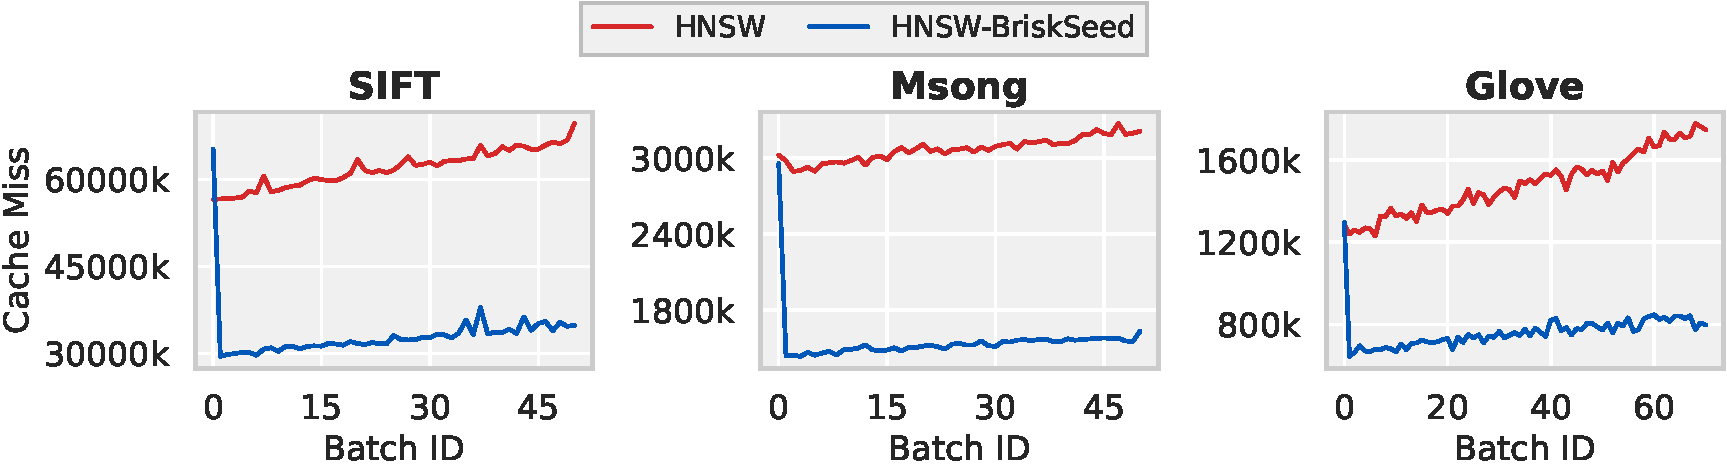
\includegraphics[width=\columnwidth]{figures/cache_miss_all.pdf}
\caption{Cache miss comparison on three datasets.}
\label{fig:cache miss results}
\end{figure}

\noindent \textbf{Parameters.} For graph-based indices, the construction beam width is all
set to $efConstruction=120$. For HNSW and SymphonyQG, the graph out-degree $M$ is set to 32, and the default search beam width is set to $efSearch=120$. For FreshDiskANN, $M=48$ and $efSearch=40$. These settings provide a balanced QPS--Recall trade-off on million-scale datasets.

\noindent \textbf{Evaluation Protocol.} For each dataset, we use 0.5 million vectors to build the initial index and treat the remaining vectors as dynamic updates, which are applied in batches of 10,000 vectors.
After each update batch, we execute the corresponding query batch and record QPS and Recall@10, following the round-based execution model of CANDOR-Bench.
Each experiment is repeated four times, and we report the average result.

% \subsection{QPS Performance and Recall}
% \begin{figure*}[t]
%     \centering
%     \subfloat[SIFT]{
%         \includegraphics[width=0.31\textwidth]{figures/sift.png}
%     }\hfill
%     \subfloat[Msong]{
%         \includegraphics[width=0.31\textwidth]{figures/msong.png}
%     }\hfill
%     \subfloat[Glove]{
%         \includegraphics[width=0.31\textwidth]{figures/glove.png}
%     }
%     \caption{QPS and Recall comparison between HNSW and HNSW-\system on three datasets.}
%     \label{fig:qps-recall-three-datasets}
% \end{figure*}

% \begin{figure*}[t]
%     \centering
%     \subfloat[QPS and recall comparisons between HNSW and HNSW-\system]{
%         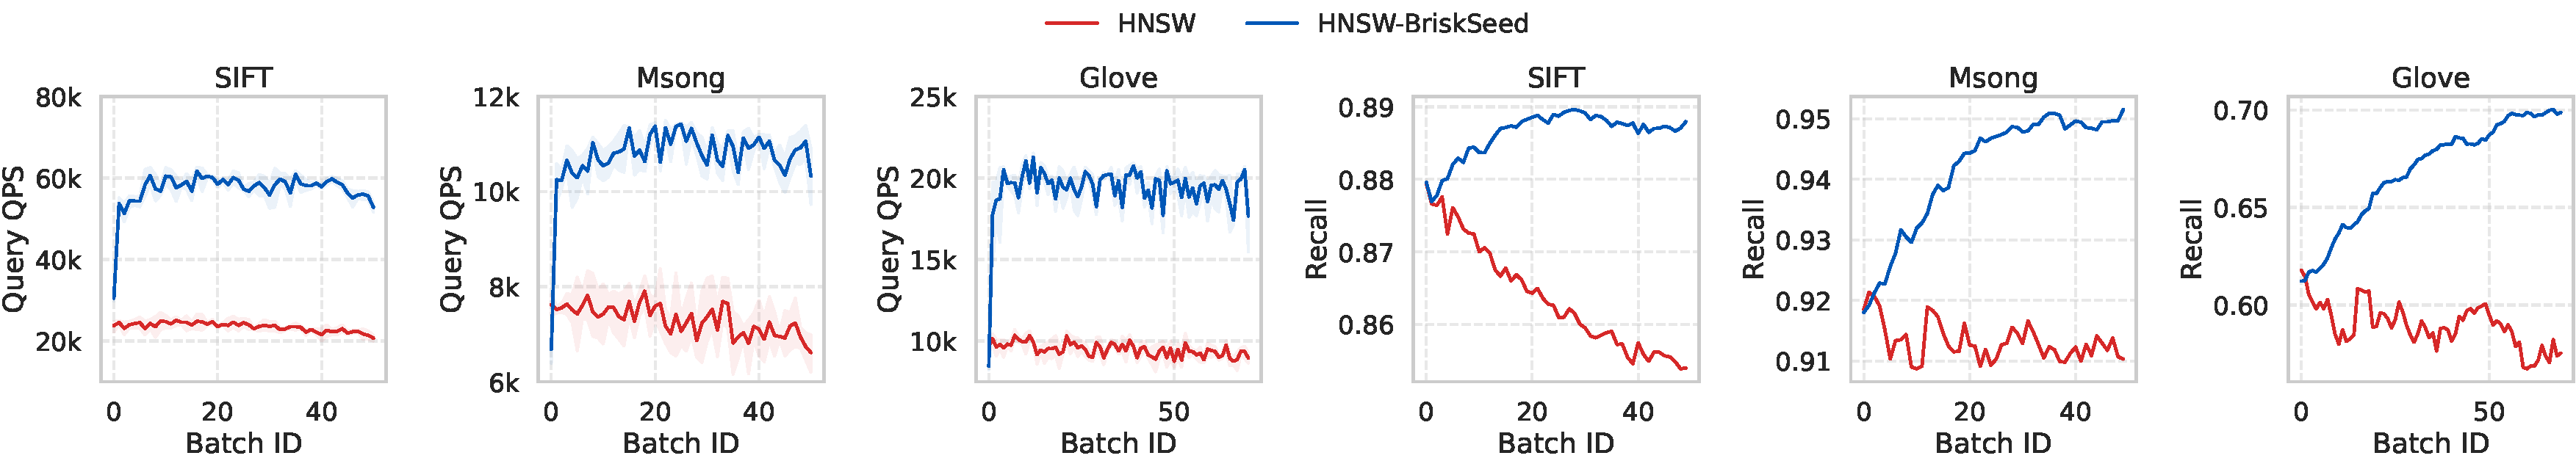
\includegraphics[width=\textwidth]{figures/qps_recall_HNSW.pdf}
%     }\hfill
%     \subfloat[QPS and recall comparisons between SymphonyQG and SymphonyQG-\system]{
%         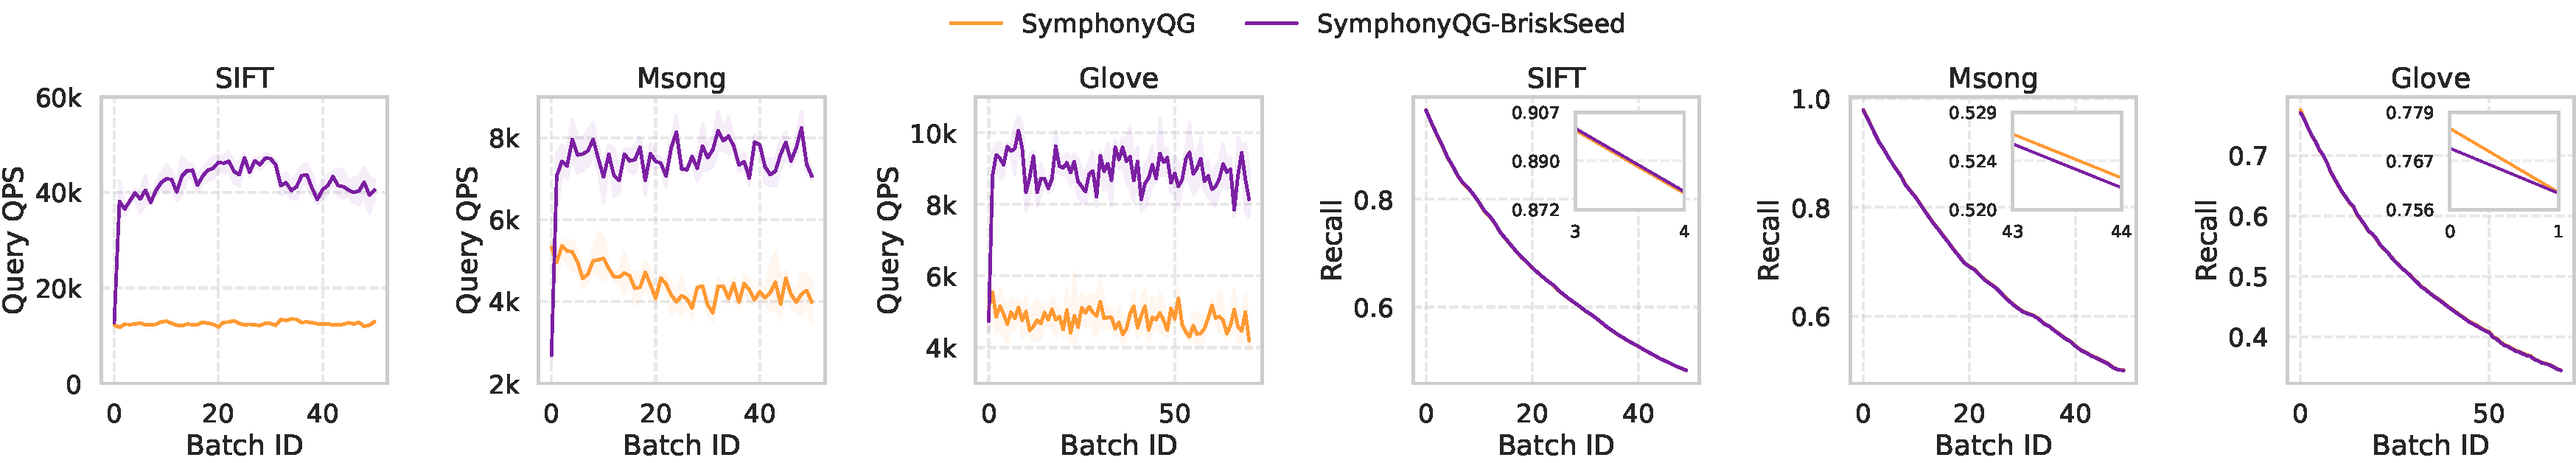
\includegraphics[width=\textwidth]{figures/qps_recall_SymQG.pdf}
%     }\hfill
%     \subfloat[QPS and recall comparisons between FreshDiskANN and FreshDiskANN-\system]{
%         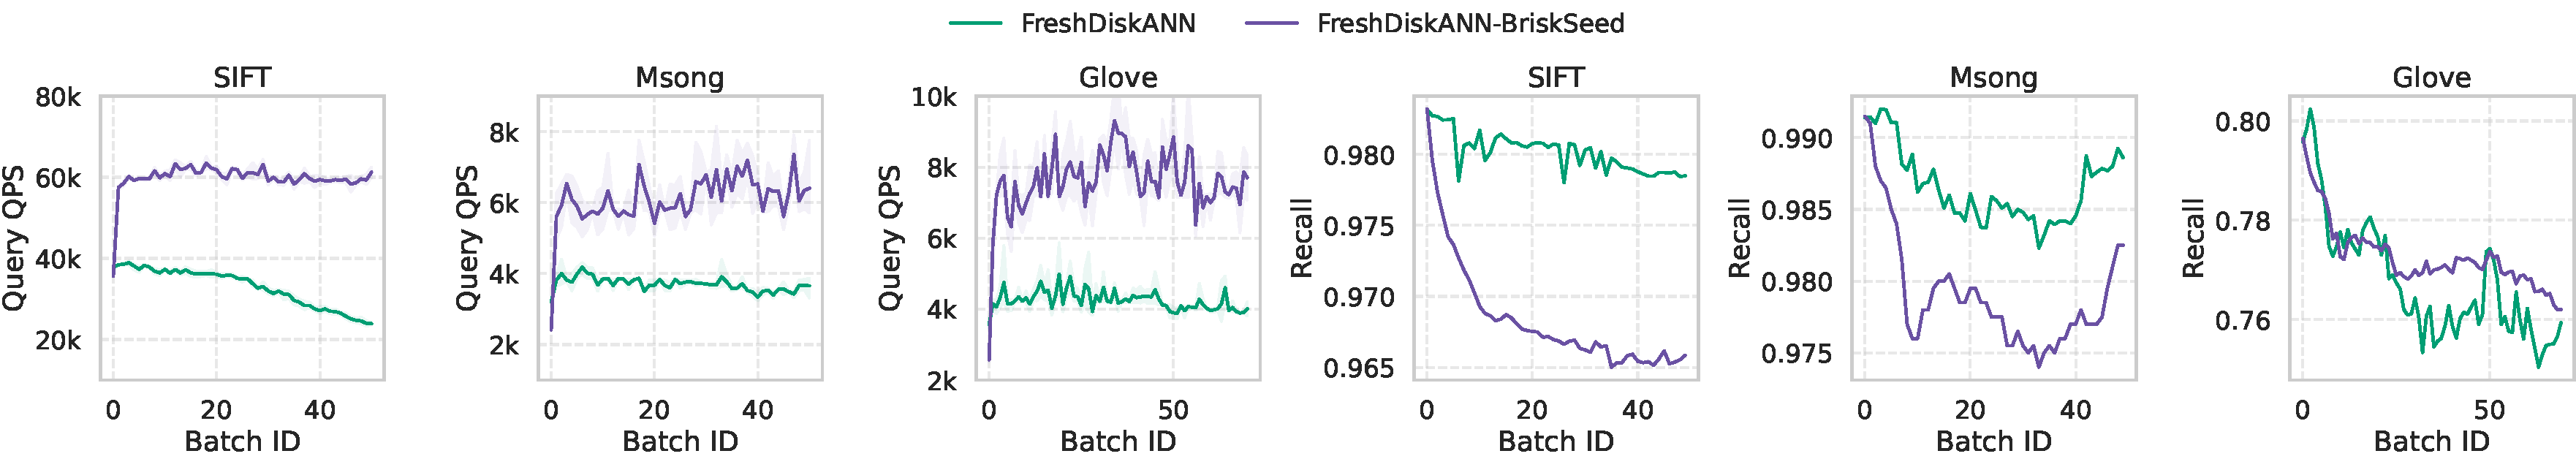
\includegraphics[width=\textwidth]{figures/qps_recall_freshdiskann.pdf}
%     }\hfill
%     \caption{QPS and Recall comparisons between baseline and baseline-\system on three datasets.}
%     \label{fig:qps-recall-three-datasets}
% \end{figure*}



% \begin{figure}[t]
% \centering
% 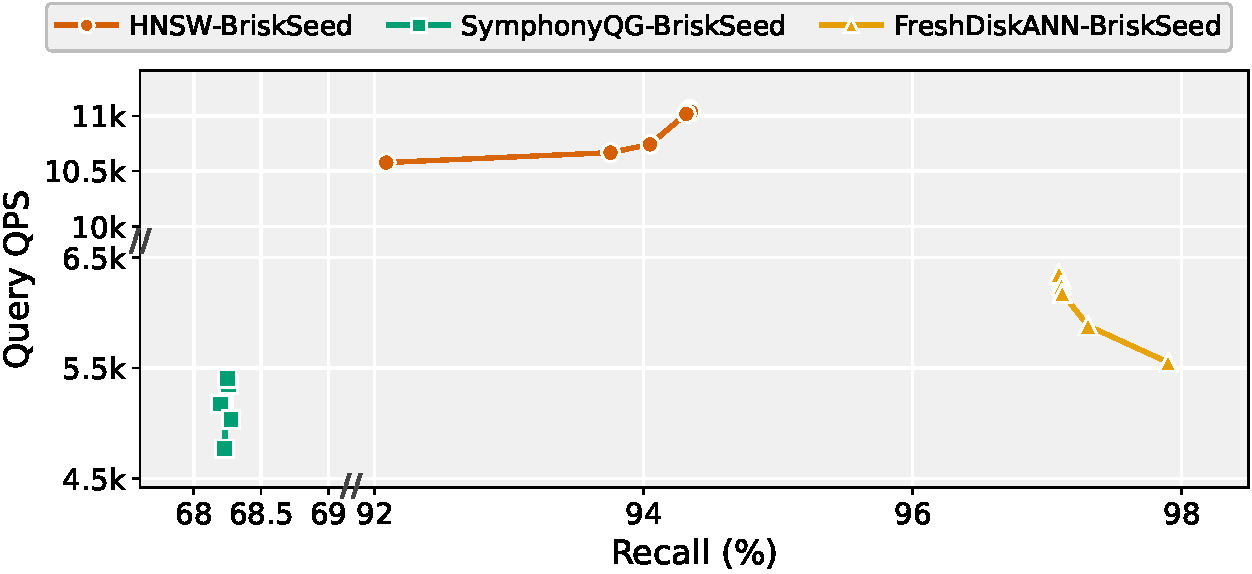
\includegraphics[width=0.85\columnwidth]{figures/hint_cons_gate_sweep_qps_recall_overlay.pdf}
% \caption{Parameter study of $\mathrm{gap}$ and $\mathrm{overlap}$ on \texttt{Msong}.}
% \label{fig:different overlap}
% \end{figure}




\subsection{Performance Study}
In this subsection, we evaluate the search performance and recall of \system, together with its impact on cache misses and memory usage.

\noindent \textbf{QPS and Recall.} Figure~\ref{fig:qps-recall-three-datasets} reports the QPS and recall trends of the baselines and their \system-enhanced variants under batch updates. The three rows correspond to HNSW, SymphonyQG, and FreshDiskANN, respectively. The left three columns show the QPS results, while the right three columns show the corresponding recall results. Overall, integrating \system consistently improves search throughput across all evaluated systems. Specifically, \system improves the QPS of HNSW, SymphonyQG, and FreshDiskANN by 1.47x--2.44x, 1.67x--3.34x, and 1.65x--1.86x, respectively. The initial surge in QPS is due to the cold start of the seed storage. These results demonstrate that \system effectively mitigates performance degradation caused by dynamic updates and substantially improves search efficiency under dynamic workloads.

These performance gains arise mainly from reduced cache misses. For example, on HNSW, \system lowers cache misses by 1.87x--1.99x across the three datasets (Figure~\ref{fig:cache miss results}). By leveraging historical seeds, \system avoids substantial graph traversals and memory accesses, which reduces cache misses and improves end-to-end query throughput.
\begin{table}[t]
    \centering
    \caption{Memory usage (in GB). Each entry shows baseline $\to$ baseline-\system, indicating the change in memory usage after deploying \system.}
    \label{tab:memory footprint}
    \begin{tabular}{lcccc}
        \toprule
        Dataset & HNSW & SymphonyQG & FreshDiskANN \\
        \midrule
        SIFT & 1.4212 $\to$ 1.4234 & 2.9933 $\to$ 2.9976   &  1.8408 $\to$ 1.8588\\
        Msong & 3.5963 $\to$ 3.5977 &  5.8832 $\to$ 5.8820 & 4.4690 $\to$ 4.4713\\
        Glove & 1.4053 $\to$ 1.4096 &  2.7819 $\to$ 2.7841 &  1.7135 $\to$ 1.7177\\
        \bottomrule
    \end{tabular}
\end{table}

\begin{figure}[t]
\centering
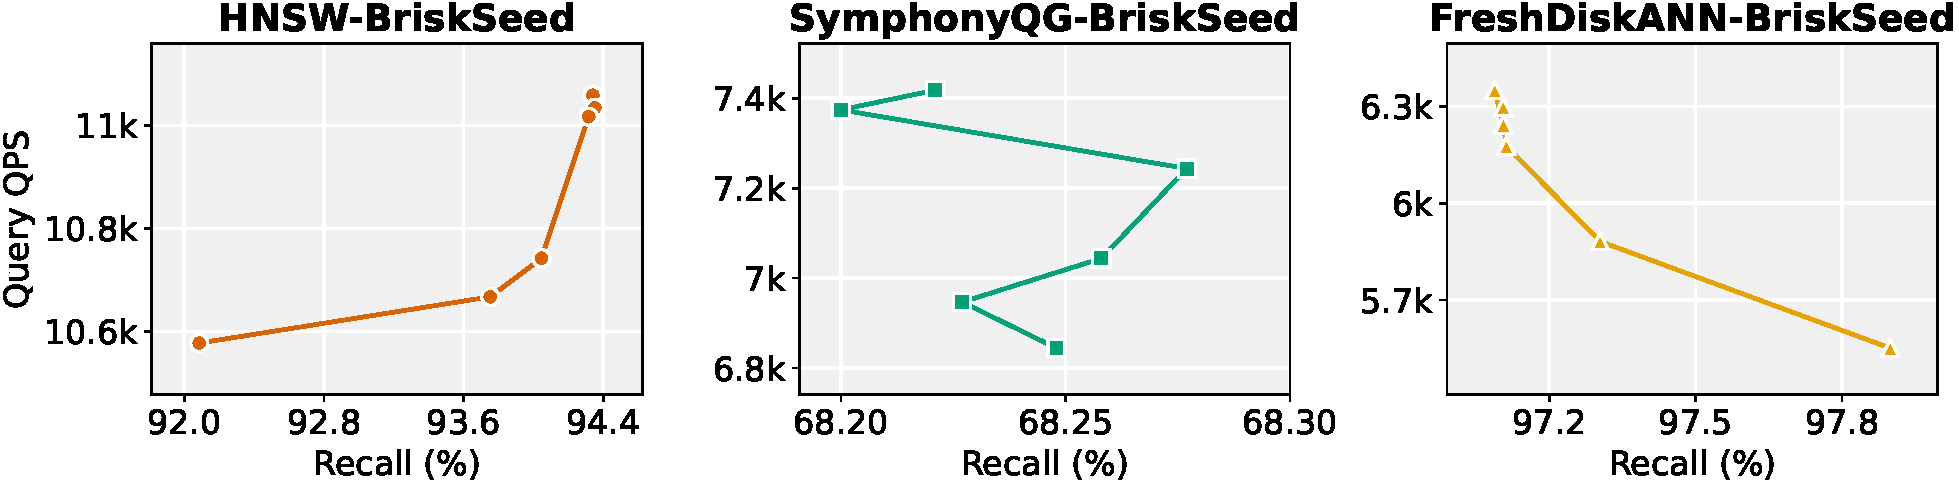
\includegraphics[width=\columnwidth]{figures/hint_cons_gate_sweep_qps_recall.pdf}
\caption{Parameter study of $\mathrm{gap}$ and $\mathrm{overlap}$ on \texttt{Msong}.}
\label{fig:different overlap}
\end{figure}

\begin{figure}[t]
\centering
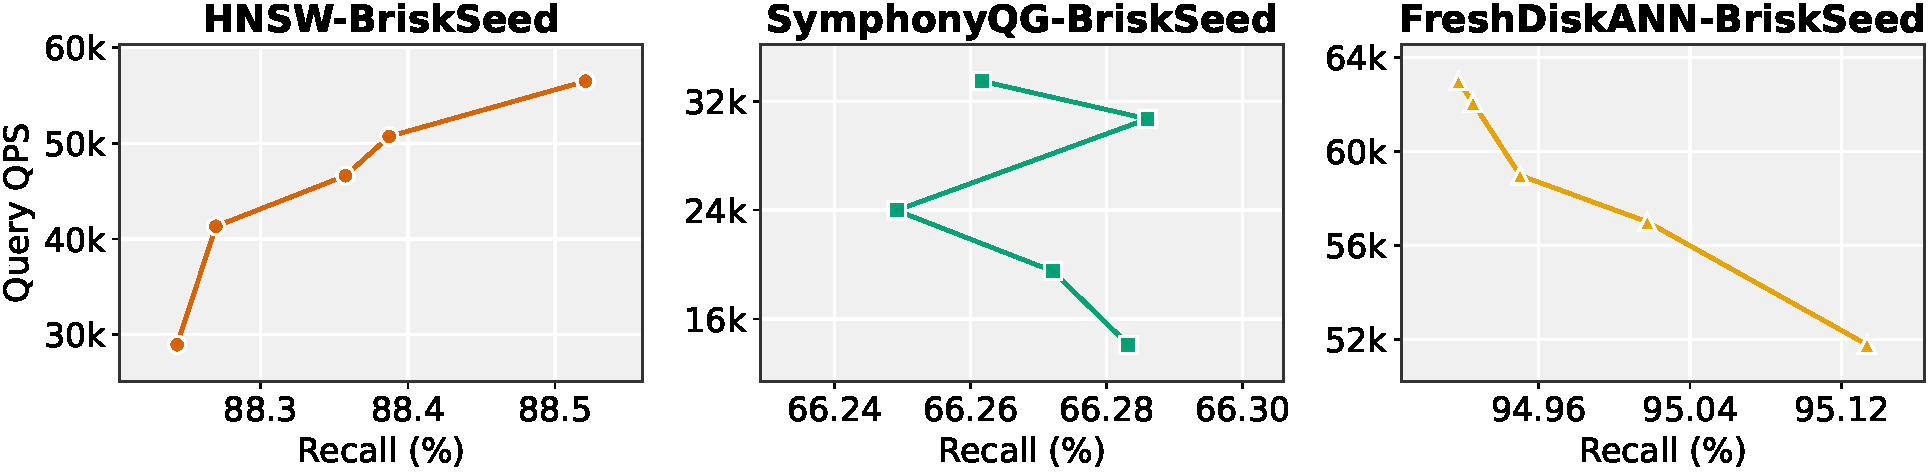
\includegraphics[width=\columnwidth]{figures/sift_hint_slot_capacity_qps_recall_subplots.pdf}
\caption{Parameter study of storage capacity on \texttt{SIFT}.}
\label{fig:different storage}
\end{figure}



In terms of recall, \system maintains comparable or even better recall in most settings. For HNSW, recall improves by 2.26\%--7.94\% across the three datasets. This is likely because dynamic updates can gradually degrade local graph neighborhoods and hierarchical links, making the standard greedy search more sensitive to suboptimal navigation paths. By reusing historical seeds, \system expands from previously effective search regions, improving candidate coverage and reducing the chance of missing true nearest neighbors.
For SymphonyQG, recall remains largely stable, varying only between -0.07\% and +0.03\%, primarily due to staleness in RabitQ codebooks under dynamic updates. For FreshDiskANN, recall changes by -1.18\% to +0.52\%, with the largest drop observed on \texttt{SIFT}. FreshDiskANN’s insertion mechanism is specifically designed to maintain neighborhood quality and recall stability through $\alpha$-pruning and structured candidate updates. In contrast, our seed-reuse local expansion, while improving search efficiency, may slightly perturb candidate exploration paths, leading to a small and bounded average recall drop without compromising overall search effectiveness. 

Overall, these results indicate that \system substantially improves search performance while preserving recall quality across different index structures and dynamic workloads.

\noindent \textbf{Memory Usage.}
Table~\ref{tab:memory footprint} shows that \system introduces negligible memory overhead across all datasets and index structures, with the maximum increase below 1\% of the original memory footprint. Since \system only maintains a lightweight seed storage and leaves the underlying index structure unchanged, its performance benefits come at marginal additional memory cost.





%We show the QPS changing curves and recall changing curves of baselines and baseline-\system variants in Figure~\ref{fig:qps-recall-three-datasets}. The horizontal rows of Figure~\ref{fig:qps-recall-three-datasets} correspond to the results of HNSW, SymphonyQG, and FreshDiskANN, respectively; the left three columns record the QPS results and the right three columns record the recall results. From this figure, we observe that after deploying \system, the search performance of HNSW, SymphonyQG, FreshDiskANN is improved by 1.47x-2.44x, 1.67x-3.34x, and 1.65x-1.86x, respectively. These results indicates the effectiveness of \system in enhancing the search performance under dynamic scenarios. Figure~\ref{fig:cache miss results} shows that taking HNSW as an example, on three datasets, the cache miss is all significantly reduced by 1.87x-1.99x after deploying \system, which leads to the search perfermance gains. Recall changes range from +2.26\% to +7.94\%, -0.07\% to +0.03\% (this is because RabitQ codebook becomes stale causing distinct recall degradation, so we show the variation in inset), and -1.18\% to 0.52\%, respectively. Only FreshDiskANN on \texttt{SIFT}, the recall is degraded by 1.18\%, while others' variations are all less than 1\%, and on HNSW, recall is all improved.

%\subsection{Ablation Study}
\begin{figure}[t]
\centering
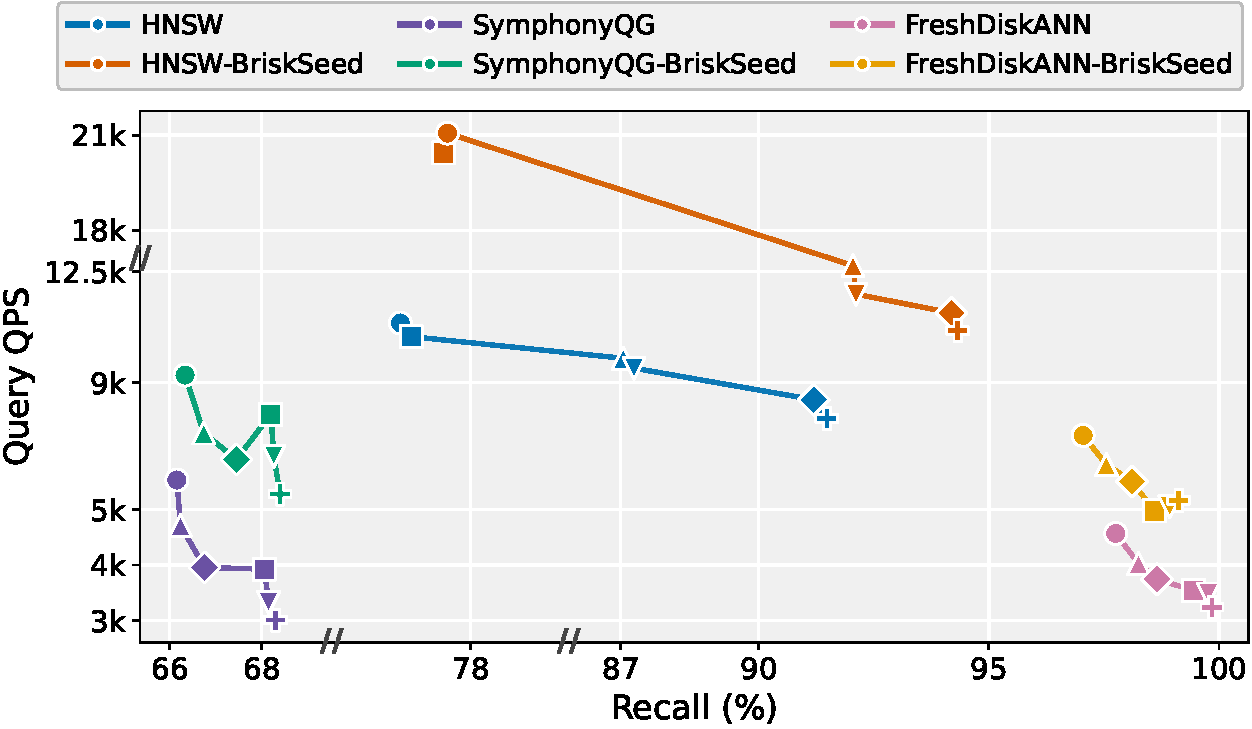
\includegraphics[width=0.85\columnwidth]{figures/msong_streamseed_hnsw_recall_qps.pdf}
\caption{Parameter study of $efSearch$ and $M$ on \texttt{Msong}.}
\label{fig:different M-ef}
\end{figure}

\subsection{Parameter Study}

\noindent \textbf{Effect of Candidate Validation Parameter $\mathrm{gap}$ and $\mathrm{overlap}$.}  We evaluate six $\mathrm{gap}$--$\mathrm{overlap}$ configurations, ranging from loose to strict validation gate, whose QPS--recall curves are shown in Figure~\ref{fig:different overlap}. Overall, stricter validation consistently reduces QPS because more queries fall back to the original search, introducing additional traversal and distance computation overhead. On HNSW-\system, SymphonyQG-\system, and FreshDiskANN-\system, QPS varies by up to 500, 640, and 800 QPS, respectively.

The recall impact depends on the relative quality of the seed-guided and original search paths. For HNSW-\system, stricter validation slightly reduces recall (up to 2.25\%) because the seed-guided path often produces better candidates than the original search under dynamic updates (Figure~\ref{fig:qps-recall-three-datasets}). Consequently, more fallbacks lead to lower overall recall. In contrast, SymphonyQG-\system exhibits highly stable recall, with variations limited to 0.07\% under different configurations. For FreshDiskANN-\system, stricter validation slightly improves recall (up to 0.81\%), indicating that its original search path remains more accurate than the seed-guided path. These results suggest that the candidate validation parameters provide an effective mechanism for balancing performance and accuracy across different index structures.

\noindent \textbf{Effect of Seed Storage Capacity.} Figure~\ref{fig:different storage} reports the QPS--recall curves under five different seed storage capacities. As the storage capacity decreases, the QPS of all three systems drops noticeably. Specifically, HNSW-\system decreases from 56,496 to 28,951 QPS, SymphonyQG-\system from 33,480 to 14,113 QPS, and FreshDiskANN-\system from 62,992 to 51,780 QPS. Nevertheless, all configurations still outperform their corresponding baselines in Figure~\ref{fig:qps-recall-three-datasets}.

The performance degradation is expected because a smaller seed storage reduces the probability of finding reusable seeds, resulting in more frequent fallback to the original search procedure. Consequently, the benefits of seed reuse become less pronounced. The recall impact remains modest, with variations of 0.28\%, 0.03\%, and 0.22\% for HNSW-\system, SymphonyQG-\system, and FreshDiskANN-\system, respectively. Similar to the observations in Figure~\ref{fig:different overlap}, the recall trend depends on the relative quality of the seed-guided and original search paths in each system.


\noindent \textbf{Effect of Index Parameter $efSearch$ and $M$.} Figure~\ref{fig:different M-ef} reports the QPS--recall curves of the three baselines and their \system-enabled variants under different $efSearch$ and $M$ settings, where points closer to the upper-right corner indicate better performance. For HNSW, we use $M \in \{16,24,32\}$ and set $efSearch$ to 40 or 120. For SymphonyQG, we use $M \in \{32,64,96\}$, and for FreshDiskANN, we use $M \in \{32,40,48\}$, with the same two $efSearch$ values.

Across these parameter settings, \system consistently improves QPS, while its impact on recall remains index-dependent and consistent with the main results in Figure~\ref{fig:qps-recall-three-datasets}: recall improves for HNSW, remains nearly unchanged for SymphonyQG, and slightly decreases for FreshDiskANN. Specifically, HNSW-\system improves QPS by 1.35x--1.95x and recall by 1.0\%--5.1\%. SymphonyQG-\system improves QPS by 1.55x--2.03x, while recall remains nearly unchanged, with only a 0.1\%--0.5\% variation. FreshDiskANN-\system improves QPS by 1.40x--1.65x, with a small recall decrease of 0.5\%--0.9\%. These results confirm that \system is robust to different index parameter $efSearch$ and $M$ choices and consistently improves the efficiency--accuracy trade-off.





\begin{figure}[t]
\centering
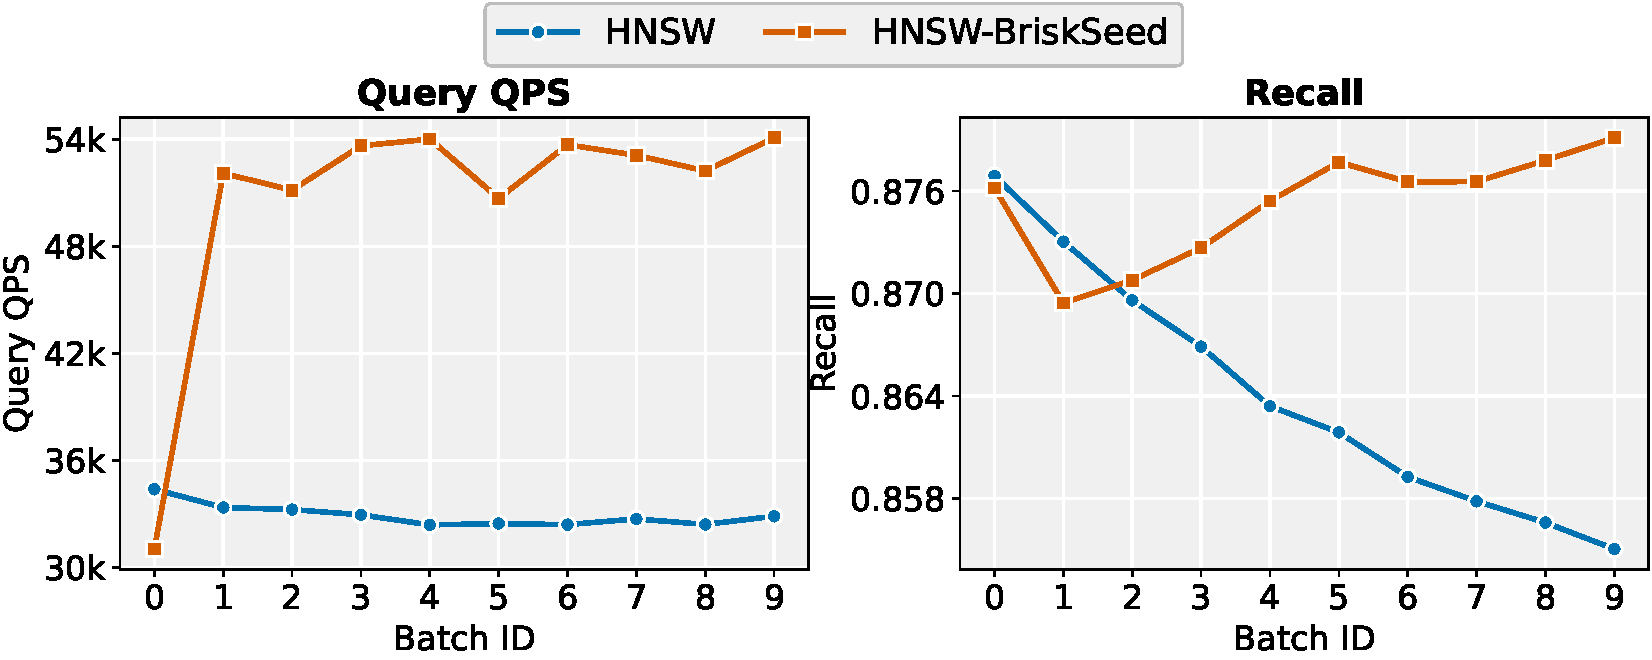
\includegraphics[width=0.9\columnwidth]{figures/sift_different_update_batches.pdf}
\caption{Scalability of \system under larger update batches on HNSW on \texttt{SIFT} (50,000 updates per batch).}
\label{fig:different update batch}
\end{figure}

\begin{figure}[t]
\centering
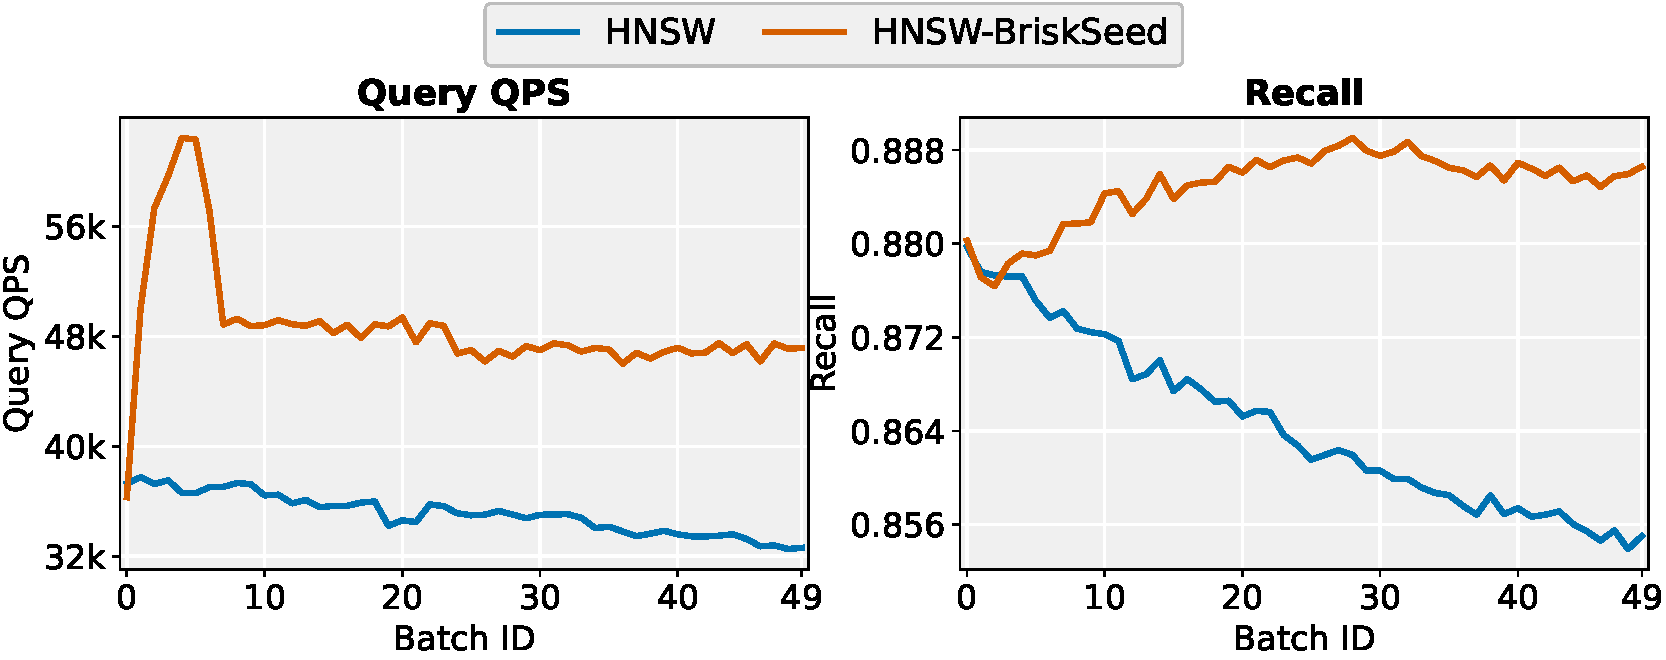
\includegraphics[width=0.9\columnwidth]{figures/sift_streamseed_hybrid_2wquery_mean.pdf}
\caption{Scalability of \system under larger and perturbed query batches on HNSW on \texttt{SIFT}.}
\label{fig:different query batch}
\end{figure}

\begin{figure}[t]
\centering
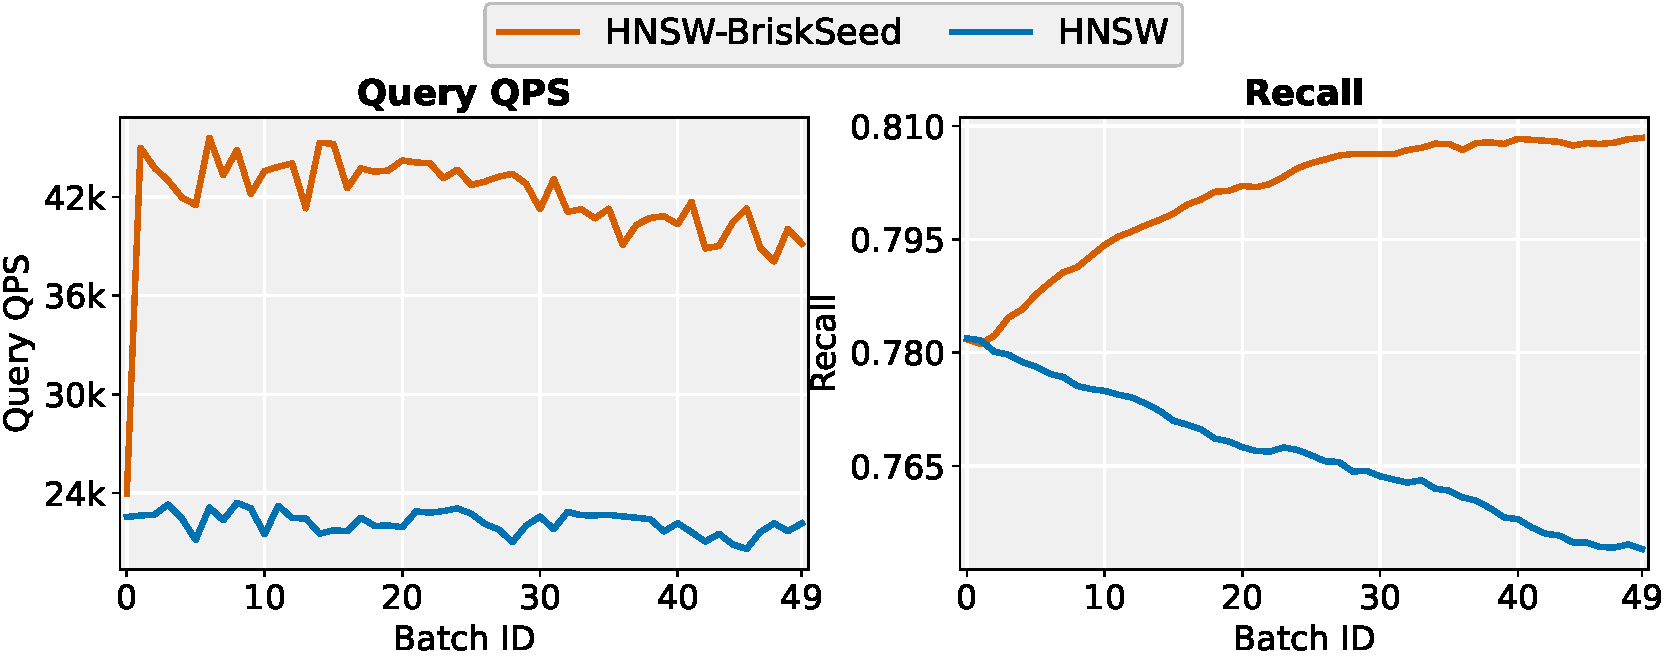
\includegraphics[width=0.9\columnwidth]{figures/sift10M_streamseed_hybrid_qps_recall.pdf}
\caption{Scalability of \system with increasing dataset scale on HNSW on \texttt{SIFT-10M}.}
\label{fig:different data}
\end{figure}

\begin{figure}[t]
\centering
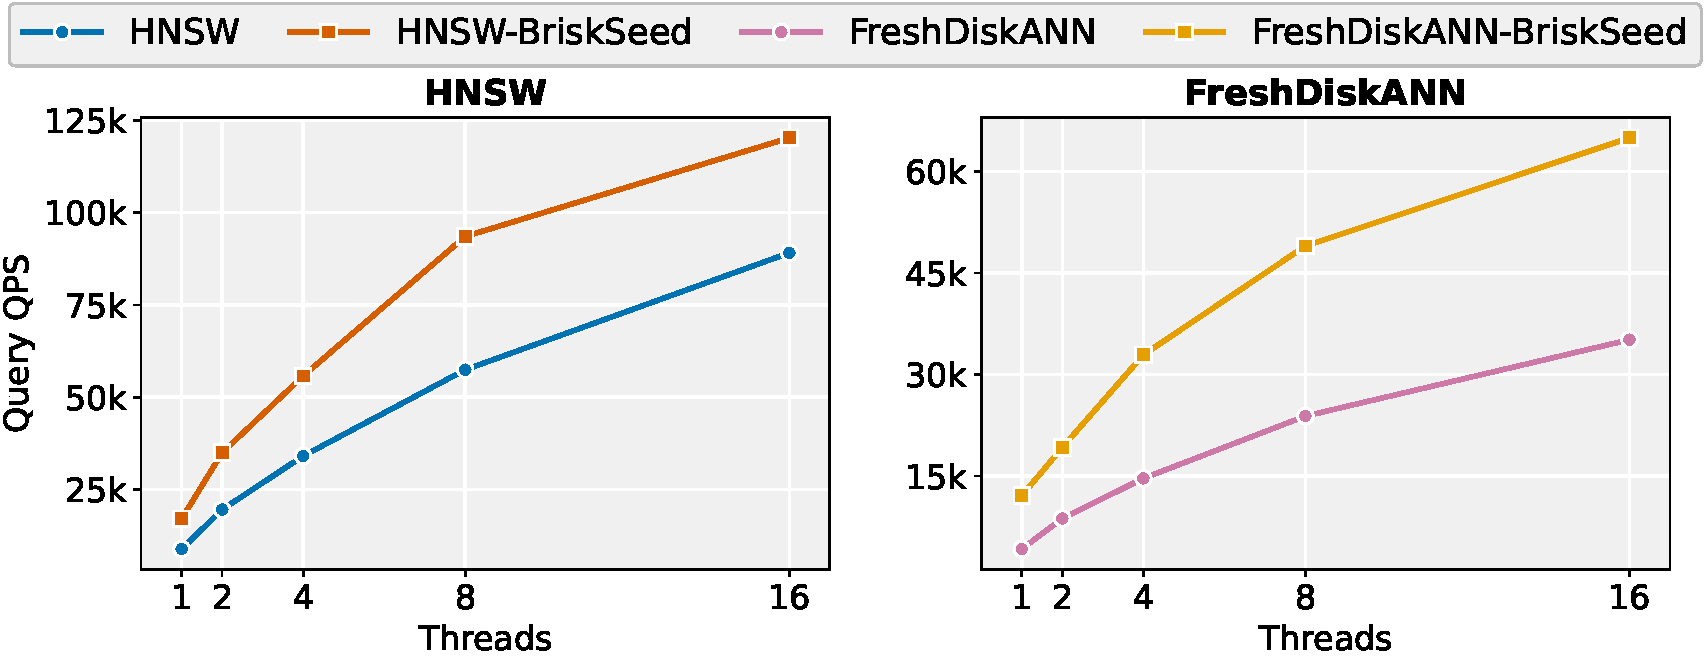
\includegraphics[width=0.9\columnwidth]{figures/sift_different_threads_qps.pdf}
\caption{Thread scaling-up evaluation on HNSW and FreshDiskANN on \texttt{SIFT}.}
\label{fig:different thread}
\end{figure}

\subsection{Scale-up Study}
This subsection evaluates \system’s performance across different update and query batch sizes, dataset scales, and thread counts.


\noindent \textbf{Update Batch Scale-up.} We evaluate the scalability of \system under larger update batches by increasing the update batch size on \texttt{SIFT} from 10,000 to 50,000 vectors. We use HNSW as the representative index. 

Figure~\ref{fig:different update batch} shows that \system remains effective at the larger batch size, improving average QPS by 1.54x and average recall by 1.12\%. These gains are lower than those under the default 10,000-vector batch setting, where QPS and recall improve by 2.24x and 2.26\%, respectively. This is mainly because larger batches cause more substantial changes to local graph neighborhoods between update rounds, making historical seeds less aligned with the current nearest-neighbor regions. Consequently, \system needs more local expansion and candidate verification, which partially reduces the QPS and recall benefits of seed reuse. Nevertheless, the results show that \system remains robust and beneficial under larger update batches.

\noindent \textbf{Query Batch Scale-up.} We also evaluate the scalability of \system under larger and perturbed query batches. Specifically, we construct a query pool of 30,000 queries from \texttt{SIFT} by introducing perturbations and noise. After each update batch, 20,000 queries are randomly sampled from the pool, ensuring that each batch contains both recurring and previously unseen queries. Figure~\ref{fig:different query batch} shows that under this setting, \system improves average QPS by 1.41x and average recall by 2.05\%. Compared with the 2.44x QPS improvement observed in the default setting on HNSW, the gain is reduced due to the increased proportion of unseen queries, which lowers the opportunity for seed reuse to some extent.

In particular, the QPS curve exhibits three phases: a rapid increase (Batch 0--5), a short decline (Batch 6--8), and a stable plateau thereafter. We attribute this behavior to the different convergence rates of seed coverage and seed quality. During the initial batches, the seed storage is rapidly populated, leading to a sharp increase in seed reuse opportunities and thus higher QPS. As the storage grows, many queries can already find matching seeds, but some of these seeds are still suboptimal and require additional local expansion and candidate validation. Consequently, the throughput gain temporarily decreases. After sufficient query batches, low-quality seeds are gradually replaced by more effective ones, allowing both seed coverage and seed quality to stabilize. As a result, the QPS converges to a stable level. These results suggest that \system can effectively adapt to query workloads with partial overlap while maintaining substantial performance benefits.



\noindent \textbf{Data Scale-up.} We further evaluate the data scalability of \system on the larger \texttt{SIFT-10M} dataset, using HNSW as the representative index. As shown in Figure~\ref{fig:different data}, \system remains effective at a larger data scale, improving QPS by 1.88x and average recall by 3.41\%. These results are consistent with the main evaluation, indicating that \system can effectively reuse historical seeds and achieve performance gains even when the index size increases. This shows that the benefits of \system are not limited to small-scale datasets, but remain robust in larger data volumes.

\noindent \textbf{Thread Scale-up.} Figure~\ref{fig:different thread} reports the query performance of HNSW and FreshDiskANN and their \system-enhanced variants using 1, 2, 4, 8, and 16 threads on the \texttt{SIFT} dataset (for SymphonyQG, we follow the single-thread configuration of the original work~\cite{Gou2025}). Across all thread counts, \system consistently improves query throughput. Specifically, improvements range from 1.35x to 1.92x for HNSW and 1.84x to 2.87x for FreshDiskANN. The highest speedups are both observed under a single-thread configuration. This is because \system reduces significant memory accesses and distance computation. In single-thread execution, these savings account for a larger fraction of total time, while in multi-thread settings, parallelism already amortizes part of the overhead, yielding slightly smaller relative gains.

